% % % % % % % % % % % % % % % % % % % % % % % % % % % % % % % % % % % % % % % % %
%
% LaTeX Presentation Template
%
% % % % % % % % % % % % % % % % % % % % % % % % % % % % % % % % % % % % % % % % %
% "THE BEER-WARE LICENSE" (Revision 42):
% Hannes Badertscher (hbaderts@hsr.ch) wrote this file. As long as you retain 
% this notice you can do whatever you want with this stuff. If we meet some day, 
% and you think this stuff is worth it, you can buy me a beer in return. 
% - Hannes Badertscher
% % % % % % % % % % % % % % % % % % % % % % % % % % % % % % % % % % % % % % % % %

\RequirePackage[l2tabu, orthodox]{nag}    % Warnings for obsolete packages
\RequirePackage{etex}                     % Load e-TeX engine
\documentclass[aspectratio=43]{beamer}    % 169 (16:9) or 43 (4:3)
\usepackage[utf8]{inputenc}               % Always use UTF-8!

\newcommand*{\Title}{A long title}
\newcommand*{\TitleShort}{Title}
\newcommand*{\Subtitle}{Subtitle}
\newcommand*{\Author}{Hannes Badertscher \newline BSc FHO in Electrical Engineering}
\newcommand*{\AuthorShort}{H.Badertscher}
\newcommand*{\Topic}{Bereich}
\newcommand*{\Lang}{en}
\newcommand*{\Institute}{institutes/ICOM-Institute_for_Communication_System_CMYK.eps}
\newcommand*{\Background}{backgrounds/Titelbild_Abend.jpg}
\newcommand*{\TocAtSection}{true}
\newcommand*{\ProgressBar}{false}

% % % % % % % % % % % % % % % % % % % % % % % % % % % % % % % % % % % % % % % % %
%
% LaTeX Presentation Template - Header File
%
% % % % % % % % % % % % % % % % % % % % % % % % % % % % % % % % % % % % % % % % %
% "THE BEER-WARE LICENSE" (Revision 42):
% Hannes Badertscher (hbaderts@hsr.ch) wrote this file. As long as you retain 
% this notice you can do whatever you want with this stuff. If we meet some day, 
% and you think this stuff is worth it, you can buy me a beer in return. 
% - Hannes Badertscher
% % % % % % % % % % % % % % % % % % % % % % % % % % % % % % % % % % % % % % % % %

% Packages
\usetheme{default}

% Fonts
\usepackage[T1]{fontenc}
\usepackage[sc]{mathpazo}               % use palatino font!
\linespread{1.05}                       % palatino needs a bit more space!
\usepackage[T1,small,euler-digits]{eulervm}
\usepackage[scaled=0.8]{beramono}       % Use bera for mono fonts
\usefonttheme{professionalfonts}        % Setup beamer to use these fonts

% Math
\usepackage{amsmath}
\usepackage{amssymb}

% Babel
\newcommand*{\LangDE}{de}
\ifx \Lang \LangDE
    \usepackage[english,ngerman]{babel}
\else
    \usepackage[ngerman,english]{babel}
\fi

% Tables
\usepackage{booktabs}
\usepackage{tabularx}
\usepackage{multicol}

% Colors
\usepackage{xcolor}
\usepackage{header/HSRColors}

% Graphics
\usepackage{epstopdf}
\usepackage{tikz}
\usetikzlibrary{arrows,backgrounds,fit,positioning,calc,shapes}
\usepackage[american currents]{circuitikz}
\usepackage{tikz-timing}[2009/12/09]
\usepackage{pgfplots}
\pgfplotsset{compat = 1.3}

% Listings
\usepackage{listings}
\usepackage{matlab-prettifier}

% SI Units
\usepackage{siunitx}
\sisetup{detect-all,sticky-per,per-mode=symbol}

% Chemical formulae
\usepackage[version=3]{mhchem}

% EToolbox for e-TeX (programming)
\usepackage{etoolbox}

% HSR Colorbox
\usepackage{tcolorbox}
\newtcolorbox{HSRBox}[1]{colback=HSRWhite,colframe=HSRBlue,title=#1}

% Setup date-time format
\usepackage{datetime}
\newdateformat{titledate}{\THEDAY.~\monthname\space\THEYEAR}


% % % % % % % % % % % % % % % % % % % % % % % % % % % % % % % % % % % % % % % % %
% Setup Document
\title[\TitleShort]{\Title}
\subtitle{\Subtitle}
\author[\AuthorShort]{\Author}

\hypersetup{
    pdftitle={\Title},
    pdfauthor={\Author},
    pdfsubject={\Subtitle},
    pdfcreator={LaTeX with hyperref and Beamer}
}

% % % % % % % % % % % % % % % % % % % % % % % % % % % % % % % % % % % % % % % % %
% Color scheme
\setbeamercolor*{frametitle}{fg=white,bg=HSRBlue}
\setbeamertemplate{section in toc}{\hspace{1em}{\scriptsize\color{HSRBlue}$\blacksquare$}~\inserttocsection}
\setbeamercolor*{section in toc}{fg=HSRSchwarz}
\setbeamercolor*{section in toc shaded}{fg=HSRSchwarz}

\setbeamertemplate{itemize item}[square]
\setbeamercolor*{itemize item}{fg=HSRBlue}
\setbeamertemplate{itemize subitem}[square]
\setbeamercolor*{itemize subitem}{fg=HSRLightGray}

\setbeamercolor{enumerate item}{fg=black}

\setbeamertemplate{caption}{\scshape\scriptsize\textcolor{HSRBlue}{\insertcaptionname:}~\insertcaption}


% % % % % % % % % % % % % % % % % % % % % % % % % % % % % % % % % % % % % % % % %
% Title page
\defbeamertemplate*{title page}{customized}[1][]{
    \setbeamertemplate{footline}{}
    \begin{tikzpicture}[remember picture,overlay,shift=(current page.south west)]

        \useasboundingbox (0,0) rectangle (\the\paperwidth,\the\paperheight);

        % Background image
        \node[anchor=south west,inner sep=0pt] at (0,0) {\includegraphics[width=\the\paperwidth]{\Background}};

        % HSR square
        \draw[draw=none,fill=HSRBlue,opacity=0.85] (6.8mm,9.1mm) rectangle (86.8mm,89.1mm);

        % HSR logo
        \draw[draw=none,fill=white] (0mm,4.5mm) rectangle (34.5mm,16.4mm);
        \node[anchor=south west,inner sep=0] at (4.5mm,4.5mm) {
\includegraphics[width=30mm]{header/HSR_Logo_RGB_72.jpg}};

        % Text
        \node[anchor=west] at (14.8mm,79.1mm) (topic){\parbox{65mm}{\color{white}\Topic}};
        \node[anchor=west, below=3mm of topic] (title) {\parbox{65mm}{\color{white}\LARGE\Title}};
        \node[anchor=west, below=1mm of title] (subtitle) {\parbox{65mm}{\color{white}\Subtitle}};

        \ifdefempty{\Institute}{}{
            \node[anchor=west, below=3mm of subtitle] (institute) {\parbox{65mm}{\includegraphics[width=40mm]{\Institute}}};
        }

        \node[anchor=west] at (14.8mm,22mm) (date) {\parbox{65mm}{\color{white}\titledate\today}};
        \node[anchor=west, above=1mm of date] (author) {\parbox{65mm}{\color{white}\Author}};

    \end{tikzpicture}
}

% % % % % % % % % % % % % % % % % % % % % % % % % % % % % % % % % % % % % % % % %
% Footer
\newcommand*{\True}{true}
\setbeamertemplate{footline}
{
    \begin{tikzpicture}
        \pgfmathparse{\paperwidth/\inserttotalframenumber*\insertframenumber}
        \pgfmathresult \let\hsrBeamerProgressWidth\pgfmathresult

        \useasboundingbox (0,0) rectangle (\the\paperwidth,1.2cm);
        \draw[color=HSRSchwarz] (0,1.2cm) -- (\the\paperwidth,1.2cm);

        \ifx \ProgressBar \True
            \draw[draw,fill] (0,1.2cm) rectangle (\hsrBeamerProgressWidth pt,1.15cm);
        \fi

        \node[inner sep=0pt,anchor=west] at (1em,0.6cm)  {
\includegraphics[width=2.5cm]{header/HSR_Logo_RGB_72.jpg}};

        \node[inner sep=0pt,anchor=center] at (0.5*\the\paperwidth,0.8cm){\scriptsize{\insertframenumber}};
        \node[inner sep=0pt,anchor=center] at (0.5*\the\paperwidth,0.4cm){\scriptsize{\AuthorShort}};

        \ifdefempty{\Institute}{}{
            \node[inner sep=0pt,anchor=east] at (\the\paperwidth-1em,0.6cm) {\includegraphics[width=3cm]{\Institute}};
        }

    \end{tikzpicture}
}

% % % % % % % % % % % % % % % % % % % % % % % % % % % % % % % % % % % % % % % % %
% TOC at beginning of every section

\ifx \TocAtSection \True
    \AtBeginSection[]
    {
        \begin{frame}<beamer>
            \frametitle{\contentsname}
            \tableofcontents[currentsection]
        \end{frame}
    }
\fi


% % % % % % % % % % % % % % % % % % % % % % % % % % % % % % % % % % % % % % % % %
\begin{document}

\frame[plain]{\titlepage}

\begin{frame}{\contentsname}
    \tableofcontents
\end{frame}

\section{First section}
\begin{frame}{Itemize}
    \begin{itemize}
        \item This is an itemize environment
        \item Nice!
        \item Even sub-items are possible
            \begin{itemize}
                \item Wow
                    \begin{itemize}
                        \item such an
                        \item awesome
                    \end{itemize}
                \item presentation!
            \end{itemize}
        \item The end.
    \end{itemize}
\end{frame}
\begin{frame}{Enumerate}
    \begin{enumerate}
        \item An item
        \item and another one
        \item Subitems:
            \begin{enumerate}
                \item This
                    \begin{enumerate}
                        \item test
                    \end{enumerate}
                \item is
                \item nice
            \end{enumerate}
        \item The end.
    \end{enumerate}
\end{frame}
\begin{frame}{Equations}
    \begin{itemize}
        \item Here, have an equation:
            \[
                \left|\int_{\Omega} Z\, d\mu\,\right| 
                \leq \int_{\Omega} |\,Z\,|\, d\mu
            \]
        \item Or something using \texttt{align}:
            \begin{align*}
                S_x &= \frac{\hbar}{2} \begin{pmatrix}
                0 & 1 \\ 1 & 0 \end{pmatrix} &
                S_y &= \frac{\hbar}{2} \begin{pmatrix}
                0 & -i \\ i & 0 \end{pmatrix} &
                S_z &= \frac{\hbar}{2} \begin{pmatrix}
                1 & 0 \\ 0 & -1 \end{pmatrix}
            \end{align*}
    \end{itemize}
\end{frame}


\section{Second section}
\begin{frame}{Boxes}
    \begin{HSRBox}{}
        Nice framed boxes also exist
    \end{HSRBox}
    \begin{HSRBox}{With \dots}
        or without title.
    \end{HSRBox}
\end{frame}
\begin{frame}{Columns and graphics}
    \begin{columns}[onlytextwidth]
        \begin{column}{0.5\textwidth}
            \begin{itemize}
                \item Multi-col environments should be made using \texttt{columns}!
                \item \emph{Never} use \texttt{minipage}'s or \texttt{multicols}.
            \end{itemize}
        \end{column}
        \begin{column}{0.5\textwidth}
            \centering
            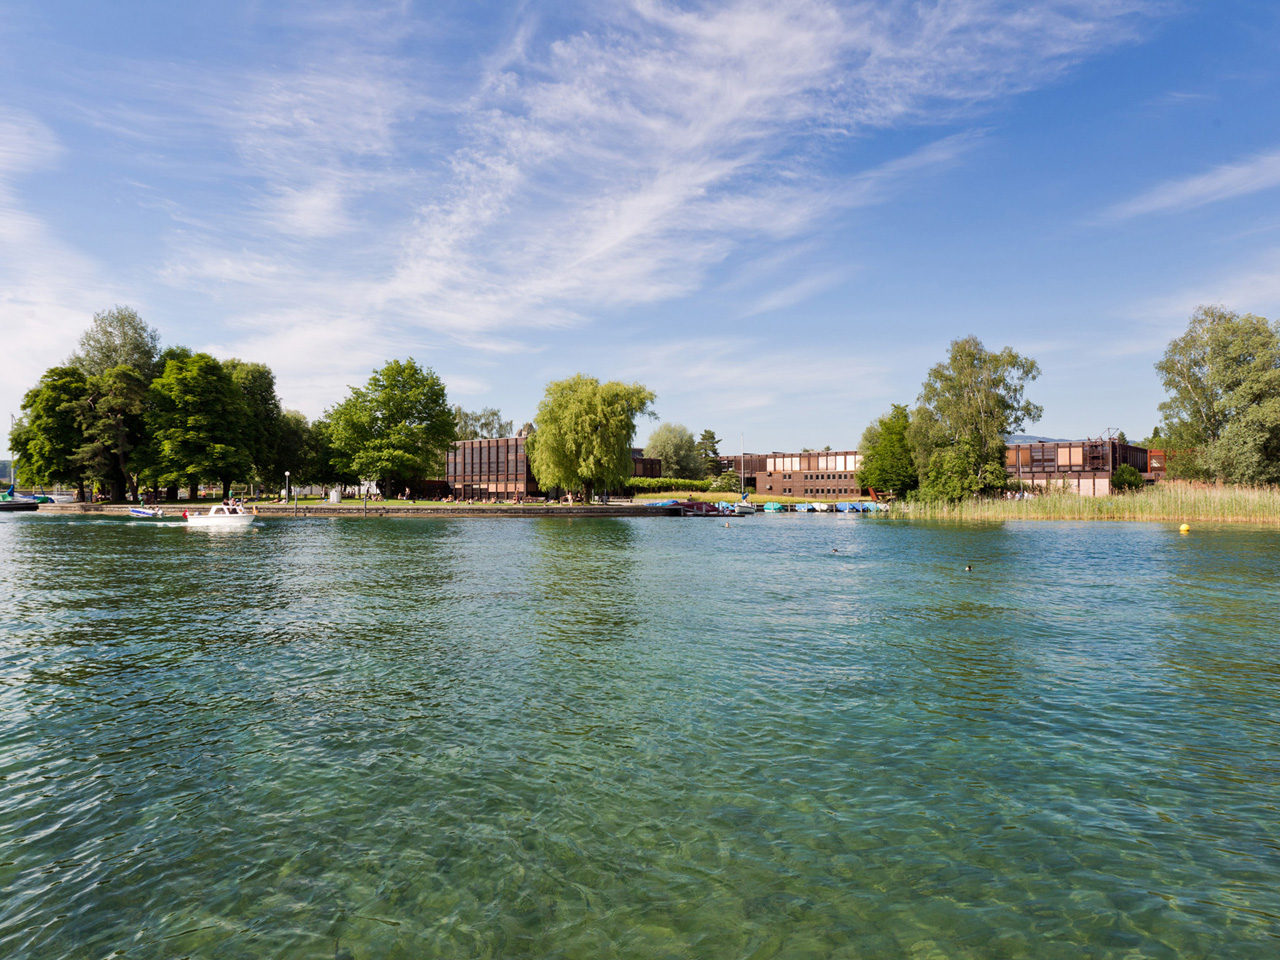
\includegraphics[width=0.8\linewidth]{backgrounds/Titelbild_Sommer.jpg}
            \captionof{figure}{A sample image. You don't need any floats here, just
            use \texttt{captionof}.}
        \end{column}
    \end{columns}
\end{frame}

\section{Last section}
\begin{frame}{A nice graphic}
    \centering
    \begin{tikzpicture}[>=latex,
    milestone/.style={circle,inner sep=2pt,draw=HSRBlue,fill=HSRBlue}
]

    % Timeline
    \draw[ultra thick,HSRBlue,->,shorten >=-6pt] (0,0) .. controls (2,0) and (6,4) .. (8,4)
    
    node[pos=0.00,milestone,fill=white] {}
    node[pos=0.18,milestone,label={[align=left]below right:Next Step}] {}
    node[pos=0.4,milestone,label={[align=left]below right:Do more\\intelligent stuff}] {}
    node[pos=0.6,milestone,label={[align=left]below right:Improve everything}] {}
    node[pos=0.8,milestone,label={[align=left]below right:Never settle}] {}
    
    ;


\end{tikzpicture}

\end{frame}
\begin{frame}{The End}
    \centering
    \LARGE That's all folks!
\end{frame}

\end{document}
% % % % % % % % % % % % % % % % % % % % % % % % % % % % % % % % % % % % % % % % %
